
\documentclass[letterpaper,twocolumn,10pt]{article}
\usepackage{usenix,epsfig,endnotes,float,enumerate}
\begin{document}

%don't want date printed
\date{}

%make title bold and 14 pt font (Latex default is non-bold, 16 pt)
\title{\Large \bf FS$^3$: FaSt File Systems, For Sure}

\author{
{\rm Jonathan Wu}\\
Harvard University
}

\maketitle

% Use the following at camera-ready time to suppress page numbers.
% Comment it out when you first submit the paper for review.
\thispagestyle{empty}


\subsection*{Abstract}
Linux file systems generally expose the same set of POSIX interface functions but make vastly different design choices on allocation, crash recovery, data organization, caching, data integrity, and more. Because many file systems are not designed to maximize performance but rather to achieve other goals, such as increased robustness, each additional feature affects performance depending on the workload. This paper evaluates ext4, XFS, Btrfs, F2FS, and ZFS, five of the most widely used Linux file systems, on sequential, random, and filebench varmail workloads. It does not declare one file system as superior, but rather demonstrates which scenarios favor which file systems and explains differences as a function of file system design. The results show that ext4 and XFS maintain strong performance as general-purpose file systems; Btrfs sacrifices significant performance for features; F2FS performs well on metadata workloads with frequent fsync calls; and ZFS performs well on sequential patterns and metadata workloads, but not on random access due to its default configuration.

\section{Introduction}

File systems sit in the kernel layer between the kernel's virtual file system (VFS) and the underlying storage device. They translate high-level I/O operations into block requests, perform consistency checks, manage file permissions, and more. Modern file systems have many jobs and, as such, are designed for different objectives. Some of them target broad compatibility and acceptable performance over a variety of access patterns, some prioritize data integrity, and others target specific workloads or hardware.

This paper is a performance study of five of the most common file systems used on Linux systems: ext4, XFS, Btrfs, F2FS, and ZFS. These represent a broad cross-section of different types of file systems, and are some of the most commonly used file systems. ext4 and XFS are general-purpose journaling file systems. Btrfs and ZFS are copy-on-write file systems. F2FS is a log-structured file system designed for flash devices. It does not attempt to rank file systems by raw speed, as there is no single speed metric that is fully representative of different workloads or needs, or that accounts for variance over a long-running operation. Instead, the paper investigates how file system features and design affect file system performance. It breaks down performance into time-series throughput and latency distributions to show a broader picture of how file systems perform in various workloads, and uses this data to explain the relationship between observed performance and file system design and mechanisms.

\section{Background}
File system performance is not usually a primary concern for choosing file systems, except in the case of workloads that handle a significant amount of small random files, where log-structured file systems have been shown to perform well. Users and system administrators often care more about reliability, access control support, transparent compression, encryption, and data integrity features. For instance, ZFS is popular with Network Attached Storage (NAS) servers as data integrity over terabytes of data is the primary concern, and speeds are often limited by network bandwidth \cite{truenas-zfs}. These features are valuable, but not free. It is helpful to understand how much performance these features cost, and where and how these performance penalties manifest.

Additionally, performance penalties manifest differently in different workloads. A file system optimized for sequential I/O may suffer in small random I/O. Copy-on-write file systems introduce additional write amplification that disproportionately affects small writes. Log-structured file systems introduce additional overhead for sequential I/O due to cleaning, but perform well in sync-heavy metadata operations due to significantly cheaper fsync calls on random I/O.

\subsection{Evaluated File Systems}
The evaluated file systems fall into three groups: general-purpose journaling file systems, integrity-oriented copy-on-write file systems, and flash-oriented log-structured file systems.
\begin{enumerate}
    \item \textbf{ext4}. ext4 is a general-purpose journaling file system used on most Linux distros as the default option. It was created to succeed ext3, adding support for extents and larger files, among other features. It focuses on being mature, highly compatible, and relatively optimized, rather than implementing unique features.
    \item \textbf{XFS}. XFS is also a general-purpose journaling file system and is designed for scalability and high throughput, with higher limits than ext4. It is the default file system for Red Hat Enterprise Linux \cite{rhel8_filesystems_overview}.
    \item \textbf{Btrfs}. Btrfs is a copy-on-write file system implementing advanced features while focusing on data integrity \cite{btrfs}. It was created to address the lack of snapshots and checksums in existing file systems.
    \item \textbf{F2FS}. F2FS is a log-structured file system designed for flash devices, taking advantage of properties specific to flash devices \cite{f2fs}. It is widely used on mobile devices with eMMC flash but also performs well on consumer and enterprise SSDs.
    \item \textbf{ZFS}. ZFS is a copy-on-write file system that also integrates volume management. Unlike the other four file systems, ZFS is hardware-aware and manages storage pools on its own, and also implements a cache that is fundamental to its design. As a file system focused on data integrity, it provides snapshots, checksums, and automatic repair that appeal to users who cannot tolerate data loss. Its settings are highly customizable, and for this paper, the default settings were used.
\end{enumerate}
\subsection{Benchmarking Challenges}
File system benchmarking is notoriously challenging. Each storage device is unique, and between user-mode testing programs and the physical NAND flash, there are many potential sources of extraneous noise and interference that must be mitigated, including device state, cache state, kernel state, CPU scheduling, background activity, measurement method, and testing interference \cite{dos_and_donts,benchmark_is_rocket_science}.

CPU scheduling and background processes introduce noise. Using test sets that fit entirely within memory measures page cache performance instead of true disk performance. Failing to precondition and age the device also produces unrealistic results by benchmarking the SSD in its most optimal state, a state that will never be reached during regular use. Running the benchmark from disk or writing logs to disk interferes with the device being tested. Finally, reporting an aggregate bandwidth number obscures the behavior of the file system while it is serving the request, which, as this paper shows, may not be as consistent as one expects.

The evaluation mitigates many of these issues by disabling access-time updates, moving non-testing processes off the CPU cores used for testing, disabling as many background and scheduled tasks as possible, disabling the swapfile, setting the workload size to be greater than the system memory size, preconditioning the disk before each run, and writing logs during testing to a RAM-backed tmpfs location before flushing to disk at the conclusion of the run. These measures ensure reproducibility on the tested machine, but due to differences in physical hardware and kernel versions, other machines may report different numbers and distributions, but the overall performance trends should be similar.

\subsection{Related Work}
Benchmarking file systems has always provided useful context, but due to hardware and software changes, past work quickly becomes obsolete. In the past decade, NVMe SSDs have become cheaper, larger, and more mainstream, and the Linux kernel has changed significantly. Due to the inherent physical differences between flash media and spinning hard drives, conclusions drawn from papers using HDDs may not hold under SSDs.

Vanninen and Wang benchmarked several file systems, including FAT32, ext2, ext3, ReiserFS, and UFS, but targeted older hardware, such as a single-core CPU and a 30 GB HDD \cite{2003-paper}. Kromer evaluated ext-family file systems, Btrfs, XFS, ReiserFS, and ZFS, but the results predate important changes in the Linux kernel (particularly, the removal of the Big Kernel Lock) and were run on older SATA SSDs \cite{2012-article}. More recent work emphasizes the need to mitigate confounding factors and explain observed differences based on file system mechanisms and designs \cite{bffs,pbfs}.

The F2FS paper is especially relevant as it compares F2FS to other file systems like ext4 and Btrfs on a variety of traces similar to the traces in this paper, showing the benefits of a flash-optimized file system \cite{f2fs}. However, the paper is over a decade old, so this paper seeks to revalidate the results of the F2FS paper on newer hardware, software, and file system implementations.

\begin{figure*}[htbp]
  \centering
  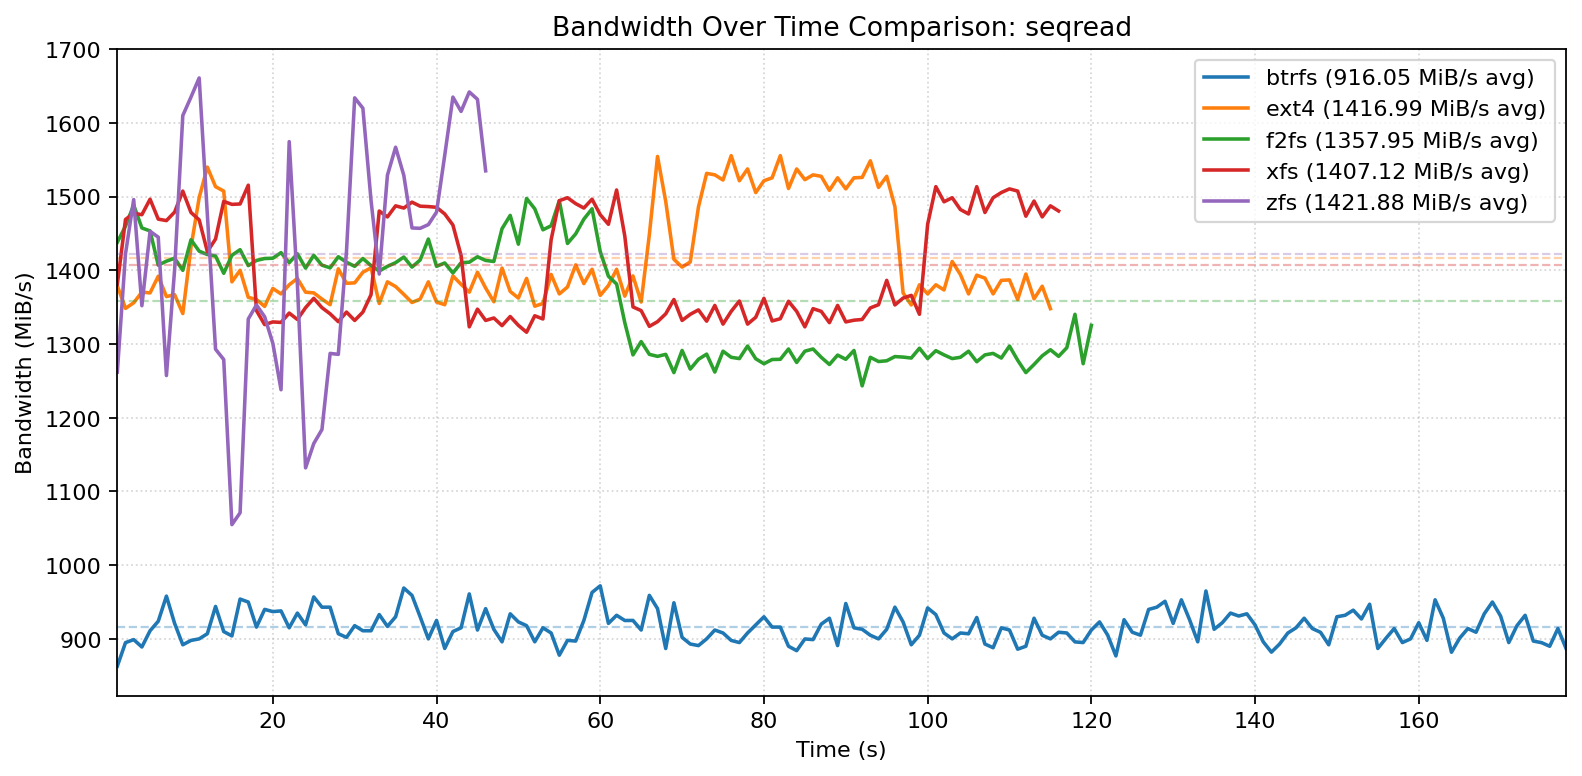
\includegraphics[width=15cm]{compare_seqread_bandwidth_over_time.png}
  \caption{Sequential read bandwidth over time for each of the tested file systems.}
  \label{fig:seqread}
\end{figure*}
\section{Evaluation}
Tests were run on an Ubuntu 24.04 server with Linux kernel 6.8.0. The machine had an 8-core Intel Xeon D-1548, 64 GB RAM, and a 2015-era 256 GB Toshiba NVMe SSD. This particular setup was chosen to avoid NUMA effects, paired with an SSD fast enough to expose file system differences.

Access time updates were disabled for all file systems to prevent hidden writes on read-only tests. ZFS caching was left enabled as default, which makes it less directly comparable to the other file systems, but because caching is an integral part of ZFS's design and is left enabled in most deployments, leaving it on makes for a more useful and representative comparison.

\subsection{Sequential Read}

Figure \ref{fig:seqread} shows that ext4, XFS, and ZFS score similarly with an average bandwidth just over 1400 MiB/s, with F2FS slightly lower, and Btrfs significantly lower. It makes sense that ext4 and XFS have consistently high bandwidths: both reflect efficient extent allocation with low overhead, maximizing the use of the device's maximum throughput. 

In ZFS's case, it would appear that checksumming is relatively cheap in sequential workloads, but its time series shows significantly higher variance than the other algorithms, which reflects the effects of its aggressive caching strategy.

F2FS's slightly slower speed can be attributed to the overhead of log-structured file systems generally. Log-structured file systems work best on small operations and only introduce additional overhead in workloads that are already sequential. , and is also observed in \cite{f2fs}. Btrfs's slow speed has been previously documented \cite{btrfs-slow}, and is likely explained by the overhead of the features and implementation compared to the more mature and optimized file systems.

\subsection{Random 4K Read}
\begin{figure*}[htbp]
  \centering
  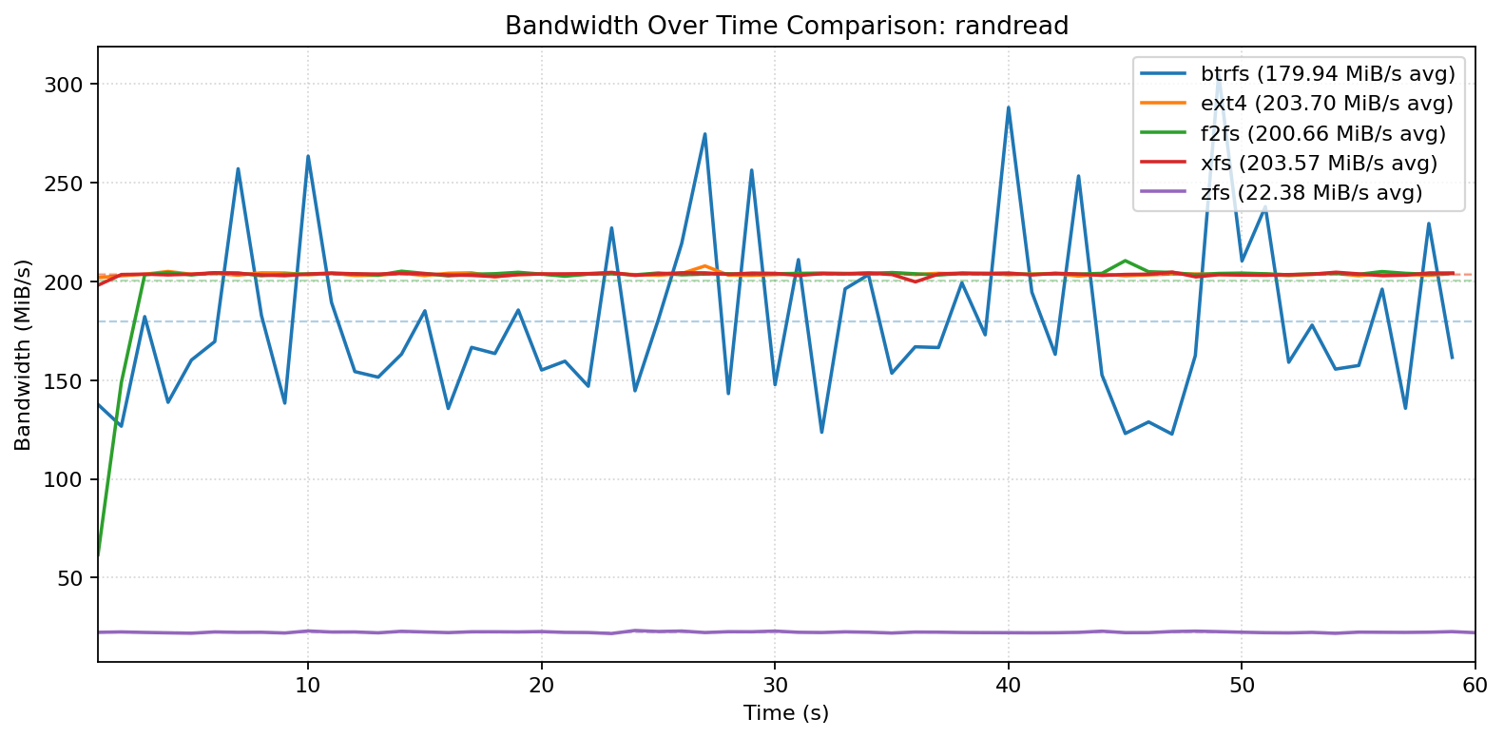
\includegraphics[width=15cm]{compare_randread_bandwidth_over_time.png}
  \caption{Random 4K read bandwidth over time for each of the tested file systems.}
  \label{fig:randread}

  \vspace{1cm}
    
  \centering
  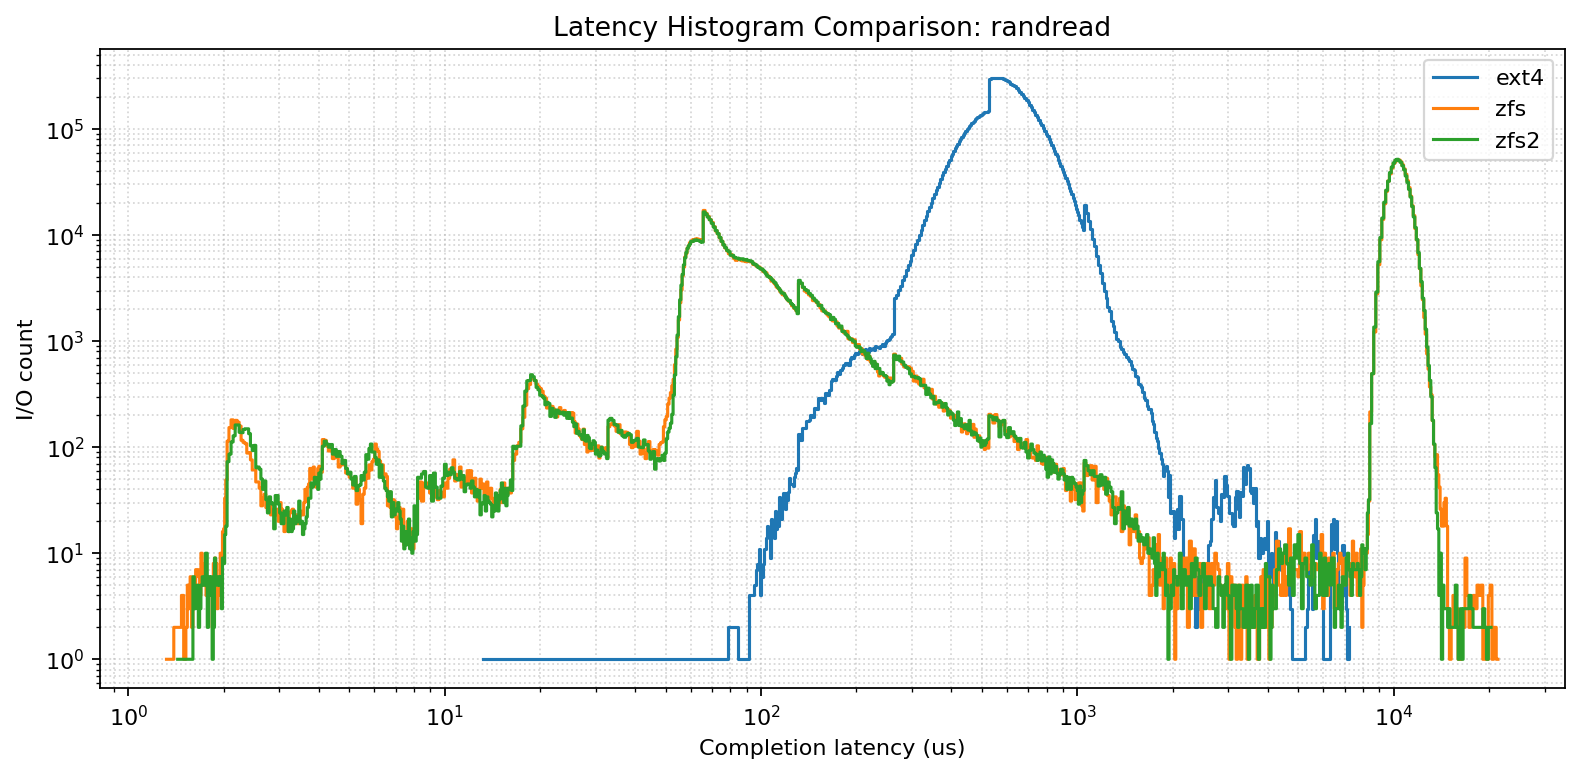
\includegraphics[width=15cm]{compare_randread_latency_histogram.png}
  \caption{Random 4K read latency for two runs of ZFS (zfs, zfs2) and one run of ext4.}
  \label{fig:randreadlatency}
\end{figure*}

Figure \ref{fig:randread} shows that all file systems except Btrfs and ZFS exhibit almost identical speeds, at 203 MB/s. Btrfs trails as a result of lower IOPS \cite{btrfs-slow}, and ZFS is significantly slower, at just 22 MB/s.

ZFS's poor performance can be attributed to its default configuration and cache behavior. ZFS uses a 128 KB block size by default (as opposed to 4 KB), and must read the entire block to check the checksum even if only 4 KB is requested, leading to a 32x read amplification when the read is a cache miss, which frequently happened given the size of the test data relative to RAM. Figure \ref{fig:randreadlatency} shows the stark differences in request latency between ext4 and two runs of ZFS taken 24 hours apart (labeled zfs, zfs2). The similarity of the two ZFS runs shows that the pattern is not random or an anomaly, but in fact a result of its caching behavior. Since ext4 does not explicitly cache reads, its latency distribution is narrower, partitioning ZFS reads to the left of the ext4 curve as fast cache hits, and ZFS reads to the right of the ext4 curve (around $10^4$ us) as expensive cache misses. If configured with a smaller block size, it would likely achieve a higher bandwidth for small reads, but at the cost of bandwidth for large sequential reads.

\subsection{Random 4K Write}
\begin{figure*}[htbp]
  \centering
  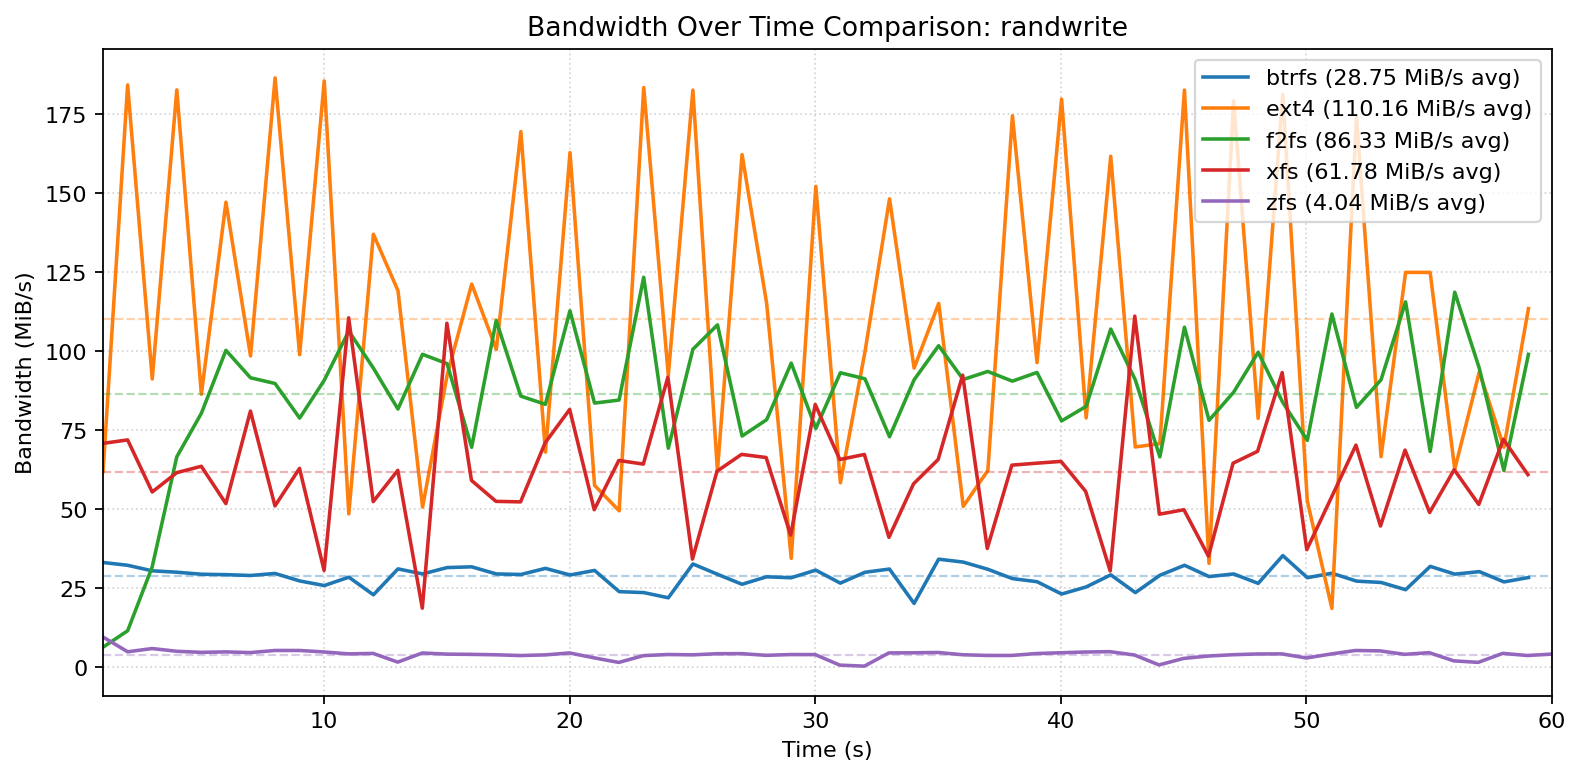
\includegraphics[width=15cm]{compare_randwrite_bandwidth_over_time.png}
  \caption{Random 4K write bandwidth over time for each of the tested file systems.}
  \label{fig:randwrite}
\end{figure*}

Random writes are particularly difficult for SSDs because they trigger device-level block invalidation and write amplification. Figure \ref{fig:randwrite} shows that compared to random reads, the speed of the fastest file system, ext4, is significantly lower and burstier. F2FS also performs well and is more consistent as a result of its log-structured design that smoothes out small updates.

Counterintuitively, ext4 beats F2FS despite not being log-structured, but this is because ext4 employs many tricks to optimize small writes, including coalescing writes, speculative allocation, and placing file data on the same erase block as its inode \cite{ext4_allocators}. XFS, the other journaling file system tested, does not perform as many tricks and thus lags behind F2FS.

ZFS again performed poorly, due to greater write amplification and the requirement to recalculate the checksum for the entire 128 KB block for each write. If tuned for small files by adjusting the block size, ZFS likely could perform on par with the faster file systems, but the default settings are tuned for larger files and thus have severe write amplification effects on small files.

\subsection{Metadata Operations}
\begin{figure}[H]
  \centering
  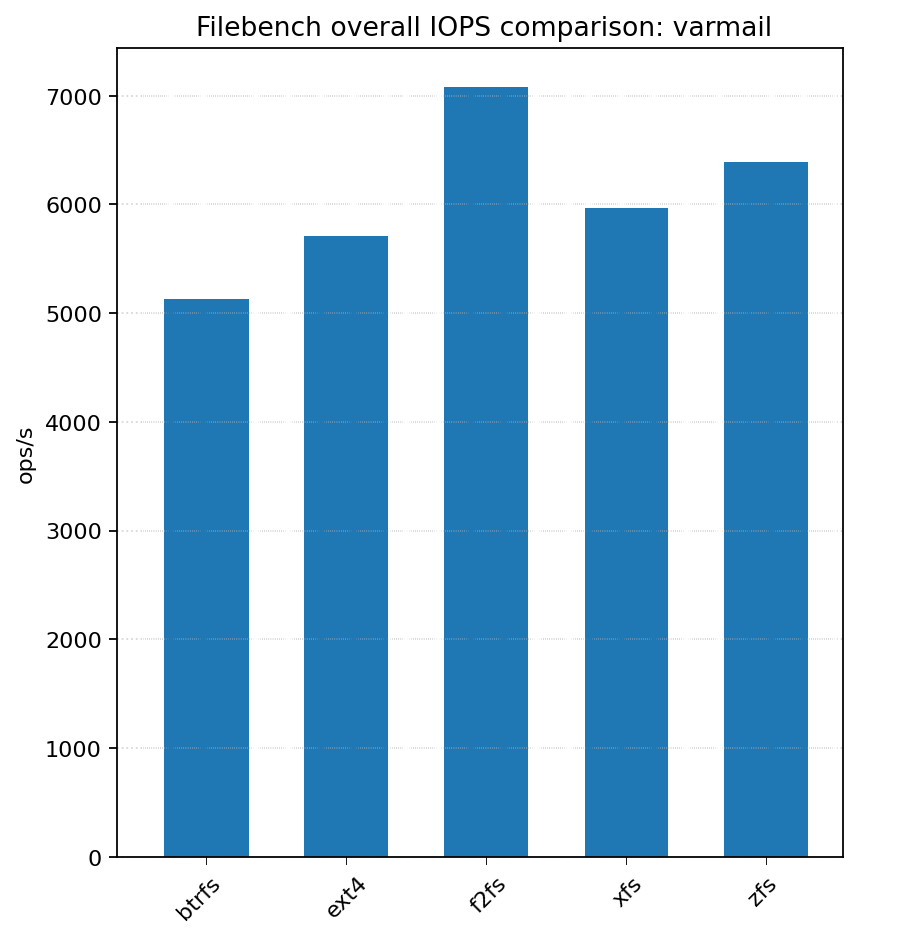
\includegraphics[width=\linewidth]{compare_varmail_filebench_iops.png}
  \caption{IOPS for each of the tested file systems on a mixed workload.}
  \label{fig:metadata}
\end{figure}
The metadata benchmark in Figure \ref{fig:metadata} runs the varmail trace in filebench, which calls the create, unlink, read, write, open, close, and fsync system calls in a loop, attempting to simulate a more realistic I/O trace. In addition to mixing read and write operations and performing metadata operations, the frequent fsync calls highlight the cost of crash-consistency.

Here, F2FS performs significantly better than its competition. Its flash-oriented and log-structured designs make fsync calls very cheap compared to the other file systems, allowing it to reduce the cost of update-heavy workloads \cite{f2fs}.

ZFS, despite performing poorly on the Random 4K read and write tests, also does well in this workload, because the I/O patterns are less random, making its cache significantly more effective and reducing the number of reads that must hit the disk.

Btrfs remains uncompetitive, and ext4, despite performing well on the synthetic benchmarks, falls behind slightly in this test as a combination of it having a higher write amplification factor than XFS and F2FS \cite{io_amp}, and the cost of fsync calls and metadata operations outweighing its small I/O optimizations.

\section{Discussion}

It is clear why ext4 or XFS are common default choices: they exhibit solid performance in all tests and are not tied to a particular type of hardware like F2FS. Their advantage is not in having a plethora of features, but rather being consistently competitive and relatively simple.

Btrfs is a prime example of extra features leading to significant performance penalties. Its benefit from advanced management features and data integrity features is outside the scope of this paper and may be useful to some, but the feature costs result in significant performance penalties. ZFS shows this too, albeit to a lesser degree. It's designed first and foremost for data integrity and large files, which make it popular for users with data integrity requirements, even though its performance is not uniformly strong, particularly with small random I/O.

ZFS also shows why average statistics do not tell the full story. With caching, excellent throughput can be achieved when many operations hit the cache, but cache misses can be very expensive and lead to long latency tails. In workloads where latency matters more than throughput, such as AWS's io2 EBS type \cite{ebs}, ZFS would likely not be a good choice.

F2FS shows the benefit of designing file systems for flash devices, especially in a world where flash storage, and particularly fast NVMe drives, are gaining market share over spinning hard drives. It does not excel at synthetic benchmarks, but shows its true benefit in a more realistic workload where its log-structured nature and awareness of flash storage design allow it to claim a higher percentage of the raw disk performance than other file systems.

The results show that file system choice can have a significant impact on some workloads, and that single numbers do not tell a complete story. Additionally, synthetic benchmarks can produce results that differ significantly from the results of more realistic simulated traces.

No file system comes out obviously on top, and when taking into account the differences in features and protections each file system provides, there is no magic formula to dictate which file system to choose. Guidance can only be given taking into account feature needs and expected workload characteristics.

\subsection{Future Work}
There is significant potential for future work, as there are many possible variations of the testing configuration. For example, if request latency is a major concern, a latency-focused analysis could be performed instead. If consistency is a major concern, additional runs with error bars could be performed.

Different mount options and feature configurations could also be compared, exploring differences as a result of:
\begin{itemize}
    \item Different hardware configurations, including different CPU types, NUMA effects, and different SSD tiers
    \item Varying ZFS's block size
    \item Selecting different journalling or cache modes
    \item Introducing RAID configurations
    \item Other simulated or real I/O traces, like SQLite, compilation, and thumbnail generation
\end{itemize}

\section{Conclusion}
No mainstream file system dominates the access pattern, and extra file system features can and do negatively impact performance to various degrees. ext4 and XFS are general-purpose file systems with strong baseline performance. Btrfs is feature-first, and as a result, has significantly worse performance. F2FS optimizes for flash device performance, and excels when data patterns (like metadata-heavy and mixed workloads) benefit from its log-structured design. ZFS offers strong data integrity, storage management features, and a unique caching system that excels in real-world tasks, but that hurts its performance in synthetic benchmarks. Choosing the correct file system should therefore start with the required features and data protection needs, and then consider access and workload patterns.

{\footnotesize \bibliographystyle{acm}
\bibliography{sample}}

%\theendnotes

\end{document}







